\documentclass[11pt]{article}
\fontfamily{times}
\usepackage{graphicx}
\usepackage{amsmath}
\usepackage{geometry}
\usepackage{subcaption}

\usepackage{natbib}

%\setcitestyle{authoryear}


\geometry{verbose,tmargin=30mm,bmargin=25mm,lmargin=25mm,rmargin=25mm}
%\newcommand{\templatefigures}[1]
{\noindent
\begin{minipage}{2cm}
\begin{center}
%\linespread{1}
%\begin{figure}
  \centering
	\vspace{-1cm}
  
\includegraphics[height = 63px]{ISI2019only_with_date_small.pdf}\\
    %\label{matrix}
%\end{figure}
\end{center}
\end{minipage}
%
\quad
%
\begin{minipage}{12cm}
\hspace*{6.8cm}
\end{minipage}
%
\quad
%
\begin{minipage}{2cm}
\begin{center}
%\linespread{1}
\vspace{-0.9cm}

\includegraphics[scale=0.4]{imag2.jpg}\\
\end{center}

\end{minipage}

\vskip0.2cm
}


\pagestyle{empty}
\begin{document}
%\templatefigures{}



\small{

\begin{center}
%The title should be centred and in bold letters. It should be informative but not too long (preferably no more than two lines).
\textbf{Model ensembles with different response variables for base and meta models: malaria disaggregation regression combining prevalence and incidence data}
\end{center}

% Model ensembles with different response variables for base and meta models:


\begin{center}
{Tim C. D. Lucas*\textsuperscript{1}; Anita Nandi\textsuperscript{1}; Michele Nguyen\textsuperscript{1}; 
Susan Rumisha\textsuperscript{1}; 
Katherine E. Battle\textsuperscript{1}; Rosalind E. Howes\textsuperscript{1}; Andre Python\textsuperscript{1}; Penny Hancock\textsuperscript{1}; Punam Someone\textsuperscript{1};
Ewan Cameron\textsuperscript{1}; Pete Gething\textsuperscript{1}; Daniel~J.~Weiss\textsuperscript{1}.}\\
{1. Malaria Atlas Project, Big Data Institute, University of Oxford, Oxford, UK - timcdlucas@gmail.com}\\ 


\end{center}
\section{Abstract}



% This is where the abstract is placed. It should include a statement about the problem being addressed in the presentation (and paper, if submitted). Continue with a discussion of why it is important to address this problem. This may be followed by some summary information about the models and methods developed and/or used to address the problem. Conclude with a description of the key results and contributions that will be covered in the presentation (and paper).\\

Maps of infection rate are one of the core tools needed for the elimination of malaria.
Reliable routine surveillance data of malaria incidence is becoming more widely available and can better measure low malaria risk than prevalence point-surveys.
However, these data are often aggregated over large, heterogeneous areas which means that they are often underpowered for learning complex relationships between the environment and malaria risk.
In contrast, prevalence point-surveys are directly linked to loval environmental conditions but are not common in many areas of the world.
A model that combines point surveys and aggregated surveillance data could have the benefits of both but must be able to account for the fact that these two data types are different malariometric units.
Here, we train multiple machine learning models on prevalence point-surveys and then combine the predictions from these with a geostatistical disaggregation model that uses routine surveillance data.
We find that, in four national case studies, using a disaggregation regression model to combine predictions from machine learning models trained on point surveys improves model accuracy relative to a baseline disaggregation regression model that uses the environmental covariates only.                                  

{\bf Keywords}: Spatial statistics; Ensemble; Stacking; Epidemiology.
}\\



\section{Introduction}


%We need to switch to downscaling models
%But they have issues of low power.
%While prevalence points should not be primary data source, they should still be used.
%One way is ML.

High-resolution maps of malaria risk are vital for control and elimination \citep{weiss2019mapping, battle2019mapping}.
However, mapping malaria in lower burden countries presents new challenges as traditional mapping of prevalence from cluster-level surveys \citep{weiss2019mapping, bhatt2017improved, battle2019mapping, bhatt2015effect} is often not effective for two reasons.
Firstly, so few individuals are infected that most surveys will detect zero cases \citep{sturrock2016mapping}.
Secondly, there is a lack of nationally representative prevalence surveys in low burden countries \citep{sturrock2016mapping, sturrock2014fine}. 
Routine surveillance data of malaria case counts, often aggregated over administrative regions defined by geographic polygons, is becoming more reliable and more widely available \citep{sturrock2016mapping} and recent work has focussed on methods for estimating high-resolution malaria risk from these data \citep{sturrock2014fine, wilson2017pointless, law2018variational, taylor2017continuous, li2012log}. 
However, the aggregation of cases over space means that the data may be relatively uninformative, especially if the case counts are aggregated over large or heterogeneous areas, because it is unclear where within the polygon, and in which environments, the cases occurred. 
This data is therefore often under-powered for fitting flexible, non-linear models as is required for accurate malaria maps \citep{bhatt2017improved, bhatt2015effect}. 
A model that combines prevalence point-surveys and aggregated surveillance data, and therefore leverages the strength of both, has great potential.

Model stacking has proven effective in many realms \citep{sill2009feature, bhatt2017improved, hao2019review}. 
Stacking improves predictions by controlling bias and variance; as long as suitably diverse models are averaged, they will have different biases while high variance in models should be averaged out even in relatively similar models.
This understanding of how stacking improves model performance indicates that diversity in models is important for stacking to be effective.
Diversity in models is typically created in two ways: by using diverse training datasets (as in Random Forests for example) and by using functionally different models (for example by averaging tree based models and neural networks).
One important trade-off in spatial modelling is whether to use local data (with a smaller sample size but that is likely to be representative of the area of study) or global data that have a larger sample size but a less close association with the areas of study.
In the context of malaria mapping, we can think about diversity of training data in this context and expect that stacking seperate models trained on local and global data will also increase the diversity of predictions in a useful way.

Here we propose training a suite of level-zero machine learning models on point-level, binomial prevalence data and stacking these models with a polygon-level, Poisson incidence model.
This modelling scheme has similarities to previous stacking methods used for malaria mapping \citep{bhatt2017improved}.
However, as the response data in the level-zero models and the stacker are on different scales (prevalence is a proportion while incidence is a rate) there are a number of important differences.
Notably, we cannot simply take a weighted average of the predictions from the level-zero models; they need to be transformed to the incidence scale and some additional flexibility to allow for mispecification of this transform needs to be allowed.
To test the effectiveness of this approach we use data from four countries: Madagascar, Colombia, Indonesia and Senegal.
We train the machine learning models on both local and global data and examine a number of different combinations of covariates: just local or global machine learning predictions, or combining the two or combining local machine learning predictions with the raw environmental covariates.
While there isn't one consistently best model, we find that in nearly all cases, using some information from local machine learning models improves model performance.


\section{Methods}

We used two data sources that reflect \emph{Plasmodium falciparum} malaria transmission; point-prevalence surveys and polygon-level, aggregated incidence data. 
We selected Madagascar, Colombia, Indonesia and Senegal as case examples as they all have fairly complete, publicly available, surveillance data at a finer geographical resolution than admin 1.
The prevalence survey data were extracted from the Malaria Atlas Project prevalence survey database using only data from 1990 onwards \citep{bhatt2015effect, guerra2007assembling, pfeffer2018ma}.
While the data cover a large time period, we did not model time explicitely but future work could include this component.
The prevalence points were then standardised to an age range of 2--10 using the model from \citep{smith2007standardizing}.

The polygon incidence data were collected from government reports and standardised using methods defined in \cite{cibulskis2011worldwide}.
This standardisation step accounts for missed cases due to lack of treatment seeking, missing case reports, and cases that sought medical attention outside the public health systems \citep{battle2016treatment}.
For reports where cases were not reported at the species level, national estimates of the ratio between \emph{P. falciparum} and \emph{P. vivax} cases were used to calculate \emph{P. falciparum} only cases. 
To minimise temporal effects we selected, for each country, one year of surveillance data. 
We used annual surveillance data from data from 2013 for Madagascar (110 districts), 2015 for Colombia (952 municipalities), 2013 for Indonesia (244 regencies and cities) and 2009 for Senegal (34 departments).
These years were selected as they had the most data in each case.


We considered an initial suite of environmental and anthropological covariates, at a resolution of approximately $5 \times 5$ kilometres that included the annual mean and log standard deviation of land surface temperature, enhanced vegetation index, malaria parasite temperature suitability index, elevation, tasseled cap brightness, tasseled cap wetness, log accessibility to cities, log night lights and proportion of urban land cover \citep{weiss2015re, weiss2018global}. 
Tasseled cap brightness and urban land cover were subsequently removed as they were highly correlated with other variables. 
The covariates were standardised to have a mean of zero and a standard deviation of one. 
These covariates were used for both the machine learning models and the polygon-level models.
Raster surfaces of population for the years 2005, 2010 and 2015, were created using data from WorldPop \citep{tatem2017worldpop} and from GPWv4 \citep{gpw4} where WorldPop did not have values. 
Population rasters for the remaining years were created by linear interpolation. 


For each country we fitted 5 models via \emph{caret} \citep{caret}: elastic net \citep{enet}, Random Forest \citep{wright2015ranger}, projection pursuit regression \citep{friedman1981projection}, neural networks \citep{nnet} and boosted regression trees \citep{gbm}.
These models were fitted to both the full malaria prevalence dataset and to more regional subsets of the data.
For Colombia we used all points from South America (locations = 522, individuals = 7,719) while for the other countries we used only data from that country (Madagascar: n = 1,505, individuals = 89,381. Indonesia: n = 4,778, individuals = 1,512,888. Senegal: n = 1,762, individuals = 80,896).
We chose these geographic regions based on a trade-off between wanting a large sample size but wanting data from geographically similar areas.
Our response variable was prevalence and we weighted the data by sample size (i.e.\thinspace the number of people tested for malaria in each survey.
For each model we ran  five-fold cross-validation to select hyperparameters using random search for Random Forest and boosted regression trees and grid search for the other models. 
Predictions from these models were then made across each country respectively.
These predictions were finally empirical logit transformed so that they are on the linear predictor scale of the top level model.
An empirical logit was used rather than a standard logit as there were many predictions of exactly zero.

The top level model was a disaggregation regression model \citep{sturrock2014fine, wilson2017pointless, law2018variational, taylor2017continuous, li2012log}.
The models were implemented and fitted using Template Model Builder \citep{TMB} in R \citep{R}.
This model is defined by a likelihood at the level of the polygon with covariates and a spatial random field at the pixel-level. 
Values at the polygon-level are given the subscript $a$ while pixel level values are indexed with $b$.

The polygon case count data, $y_a$ is given a Poisson likelihood
$$y_a \sim \operatorname{Pois}(i_a\mathrm{pop_a})$$
where $i_a$ is the estimated polygon incidence rate and $\mathrm{pop_a}$ is the observed polygon population-at-risk. 
This polygon-level likelihood is linked to the pixel level prevalence 
$$i_a = \frac{ \sum(i_b \mathrm{pop}_b)}{\sum  \mathrm{pop}_b} $$
$$i_b = \mathrm{p2i}(p_b)$$
where $\mathrm{p2i}$ is from a model that was published previously \citep{cameron2015defining} which defines a function
$$\mathrm{p2i}: f(P) = 2.616P - 3.596P^2 + 1.594P^3.$$
The fact that the model passes through prevalence space ensures that the predictions from the machine learning models can be appropriately scaled.
The linear predictor of the model is related to prevalence by a typical logit link function and includes an intercept, $\beta_0$, covariates, $X$, with regression parameters $\beta$, a spatial, Gaussian, random field, $u_s(\rho, \sigma_u)$, and an \emph{iid} random effect, $v_j(\sigma_v)$.
$$p_b = \operatorname{logit}^{-1}\left(\beta_0 + \beta X  + u_s(\rho, \sigma_u) + v_j(\sigma_v)\right)$$
The Gaussian spatial effect has a Mat\'ern covariance function and two hyperparameters: $\rho$, the nominal range (beyond which correlation is $< 0.1$) and $\sigma_u$, the marginal standard deviation.
The \emph{iid} random effect models both missing covariates and extra-Poisson sampling error.

Finally, we complete the model by setting priors on the parameters $\beta_0, \beta, \rho$ and $\sigma_u$ and $\sigma_v$. 
We assigned $\rho$ and $\sigma_u$ a joint penalised complexity prior \citep{fuglstad2018constructing} such that $P(\rho < 1) = 0.0001$ (except for Indonesia where we set $P(\rho < 3) = 0.0001$ due to it's much larger size) and $P(\sigma_u > 1) = 0.0001$. 
This prior encoded our \emph{a priori} preference for a simpler, smoother random field.
We set this prior such that the random field could explain most of the range of the data if required.

We assigned $\sigma_v$ a penalised complexity prior \citep{simpson2017penalising} such that $P(\sigma_v > 0.05) =  0.0001$. 
This was based on a comparison of the variance of Poisson random variables, with rates given by the number of polygon-level cases observed, and an independently derived upper and lower bound for the case counts using the approach defined in \citep{cibulskis2011worldwide}. 
We found that an \emph{iid} effect with a standard deviation of 0.05 would be able to account for the discrepancy between the assumed Poisson error and the independently derived error.

Finally, we set different priors on the regression coefficients depending on which covariates were used.
When environmental covariates or a mix of environmental covariates and predictions from machine learning models were used we set the prior to be weakly regularising, $\beta_i \sim \operatorname{ Norm}(0, 0.4)$, such that it is unlikely that any single covariate could explain the full range of the response data.
When only machine learning model predictions were used we set $\beta_i \sim \operatorname{ Norm}(\frac{1}{M}, 0.4)$ where $M$ is the number of machine learning models being used. 
This prior  sets our \emph{a priori} expectation that all the machine learning prediction models are positively and equally correlated with incidence i.e. this prior encodes standard model averaging.
It is important to note that this setup does not constitute true stacking in which we would enforce $\sum_i \beta_i = 1$ \citep{bhatt2017improved}.
In a preliminary analysis we tested the case where we force $\beta_i > 0$ which in practice is largely the same as the $\sum_i \beta_i = 1$  \citep{breiman1996stacked} but allows a small amount of flexibility to handle mispecification in $\mathrm{p2i}$.
This analysis did not find any benefits to this approach so it was not considered further.



We compared the performance of the models with five sets of covariates, $X$.
Firstly, we used the environmental and anthropogenic covariates, centered and standardised as a baseline model (subsequantly called Enviro).
Secondly, we used the predictions from the machine learning models trained on local data (ML\textsubscript{l}).
Thirdly, we combined the predictions from the machine learning models and the environmental coviarates in one model (Enviro + ML\textsubscript{l}).
Fourthly, we used predictions from the machine learning models trained on the global data (ML\textsubscript{g}).
Finally, we combined predictions from the machine learning models trained on regional data and global data (ML\textsubscript{l} + ML\textsubscript{g}).

To compare the five models we used two cross-validation schemes. 
In the first, polygon incidence data was randomly split into six cross-validation folds.
In the second, polygon incidence data was split spatially into k folds (via k-means clustering on the polygon centroids).
We set k as 3 for Madagascar and Colombia.
Due to its large size we set k as 7 for Indonesia.
Due to the small sample size, we set k as 5 for Senegal.
This spatial cross-validation scheme is testing the models' ability to make predictions far from data where the spatial random field is not informative.
Our primary performance metric was correlation between observed and predicted data.
We also examined the calibration of models by calculating the proportion of held out data that were within their 80\% credible intervals.


\section{Results}

Figures~\ref{f:scatter1} and \ref{f:scatter2} show the model performance under random and spatial cross-validation for all countries. 


%\begin{table}[h!]
%\caption{Pearson correlations between observed and predicted values. }
%\centering
%\begin{tabular}{llrrr}
%Cross-validation scheme & Country &  Covariates &  ML &  Covs + ML \\
%\hline 
% Random &  Colombia &  0.45 &  \textbf{0.55} &  0.54 \\
% Random &  Madagascar &  0.70 &  \textbf{0.76} &  0.75 \\
% Spatial &  Colombia &  0.05 &  \textbf{0.18} &  0.10 \\
% Spatial &  Madagascar &  0.22 &  \textbf{0.63} &  0.61 
%\end{tabular}
%\label{t:results}
%\end{table}


\begin{table}[h!]
\caption{Pearson correlations between observed and predicted values. }
\centering
\begin{tabular}{llrrrr}
Country &  Cross-validation & Enviro &  ML\textsubscript{l} &  Enviro + ML\textsubscript{l} \\
\hline 
 Colombia & Random &  0.59 & 0.59 & \textbf{0.61} \\
 Colombia &  Spatial &  0.12 &  \textbf{0.33} &  0.25\\
 Madagascar & Random &   0.70 &  \textbf{0.73} & 0.69 \\
 Madagascar &  Spatial &  0.22 &  \textbf{0.66} & 0.18\\
 Senegal &  Random &  \textbf{0.58} &  0.51 & 0.57 \\
 Senegal &  Spatial &  \textbf{0.63} &  0.27 &  \textbf{0.63} \\
 Indonesia &  Random &  0.52 &  0.48 &  \textbf{0.59} \\
 Indonesia &  Spatial &  0.45 &  0.44 &  \textbf{0.51} \\
\end{tabular}
\label{t:results}
\end{table}





\begin{table}[h!]
\caption{Pearson correlations between observed and predicted values. }
\centering
\begin{tabular}{llrrrr}
Country &  Cross-validation & Enviro &   ML\textsubscript{g} & ML\textsubscript{l} + ML\textsubscript{g} \\
\hline 
 Colombia & Random &  \textbf{0.59} &0.58 & 0.56 \\
 Colombia &  Spatial &  0.12 &  0.18 & \textbf{0.34}\\
 Madagascar &  Random &  0.70 &  0.70 & \textbf{0.71} \\
 Madagascar &  Spatial &  0.22 &  \textbf{0.63} & 0.60\\
 Senegal &  Random &  \textbf{0.58} &  0.30 & 0.08 \\
 Senegal &  Spatial &  \textbf{0.63} & 0.36 & 0.35 \\
 Indonesia &  Random &  \textbf{0.52} & 0.46 & 0.32 \\
 Indonesia &  Spatial &  \textbf{0.45} & 0.41 & \textbf{0.45} \\
\end{tabular}
\label{t:results2}
\end{table}


%\begin{table}[h!]
%\caption{Pearson correlations between observed and predicted values. }
%\centering
%\begin{tabular}{llrrrr}
%Cross-validation scheme & Country &  Covariates &  ML\textsubscript{l} &  ML\textsubscript{g} & ML\textsubscript{l} + ML\textsubscript{g} \\
%\hline 
% Random &  Colombia & \textbf{0.59} & \textbf{0.59} &  0.58 & 0.56 \\
% Random &  Madagascar &  0.70 &  \textbf{0.73} &   0.70 & 0.71 \\
% Random &  Senegal &  \textbf{0.58} &  0.51 &  0.30 & 0.08 \\
% Random &  Indonesia &  \textbf{0.52} &  0.48 &  0.46 & 0.32 \\
% Spatial &  Colombia &  0.12 &  0.33 &  0.18 & \textbf{0.34}\\
% Spatial &  Madagascar &  0.22 &  \textbf{0.66} &  0.63 & 0.60\\
% Spatial &  Senegal &  \textbf{0.63} &  0.27 &  0.36 & 0.35 \\
% Spatial &  Indonesia &  \textbf{0.45} &  0.44 &  0.41 & \textbf{0.45} \\
%\end{tabular}
%\label{t:results}
%\end{table}

% to do table of coverage.


\begin{figure}
  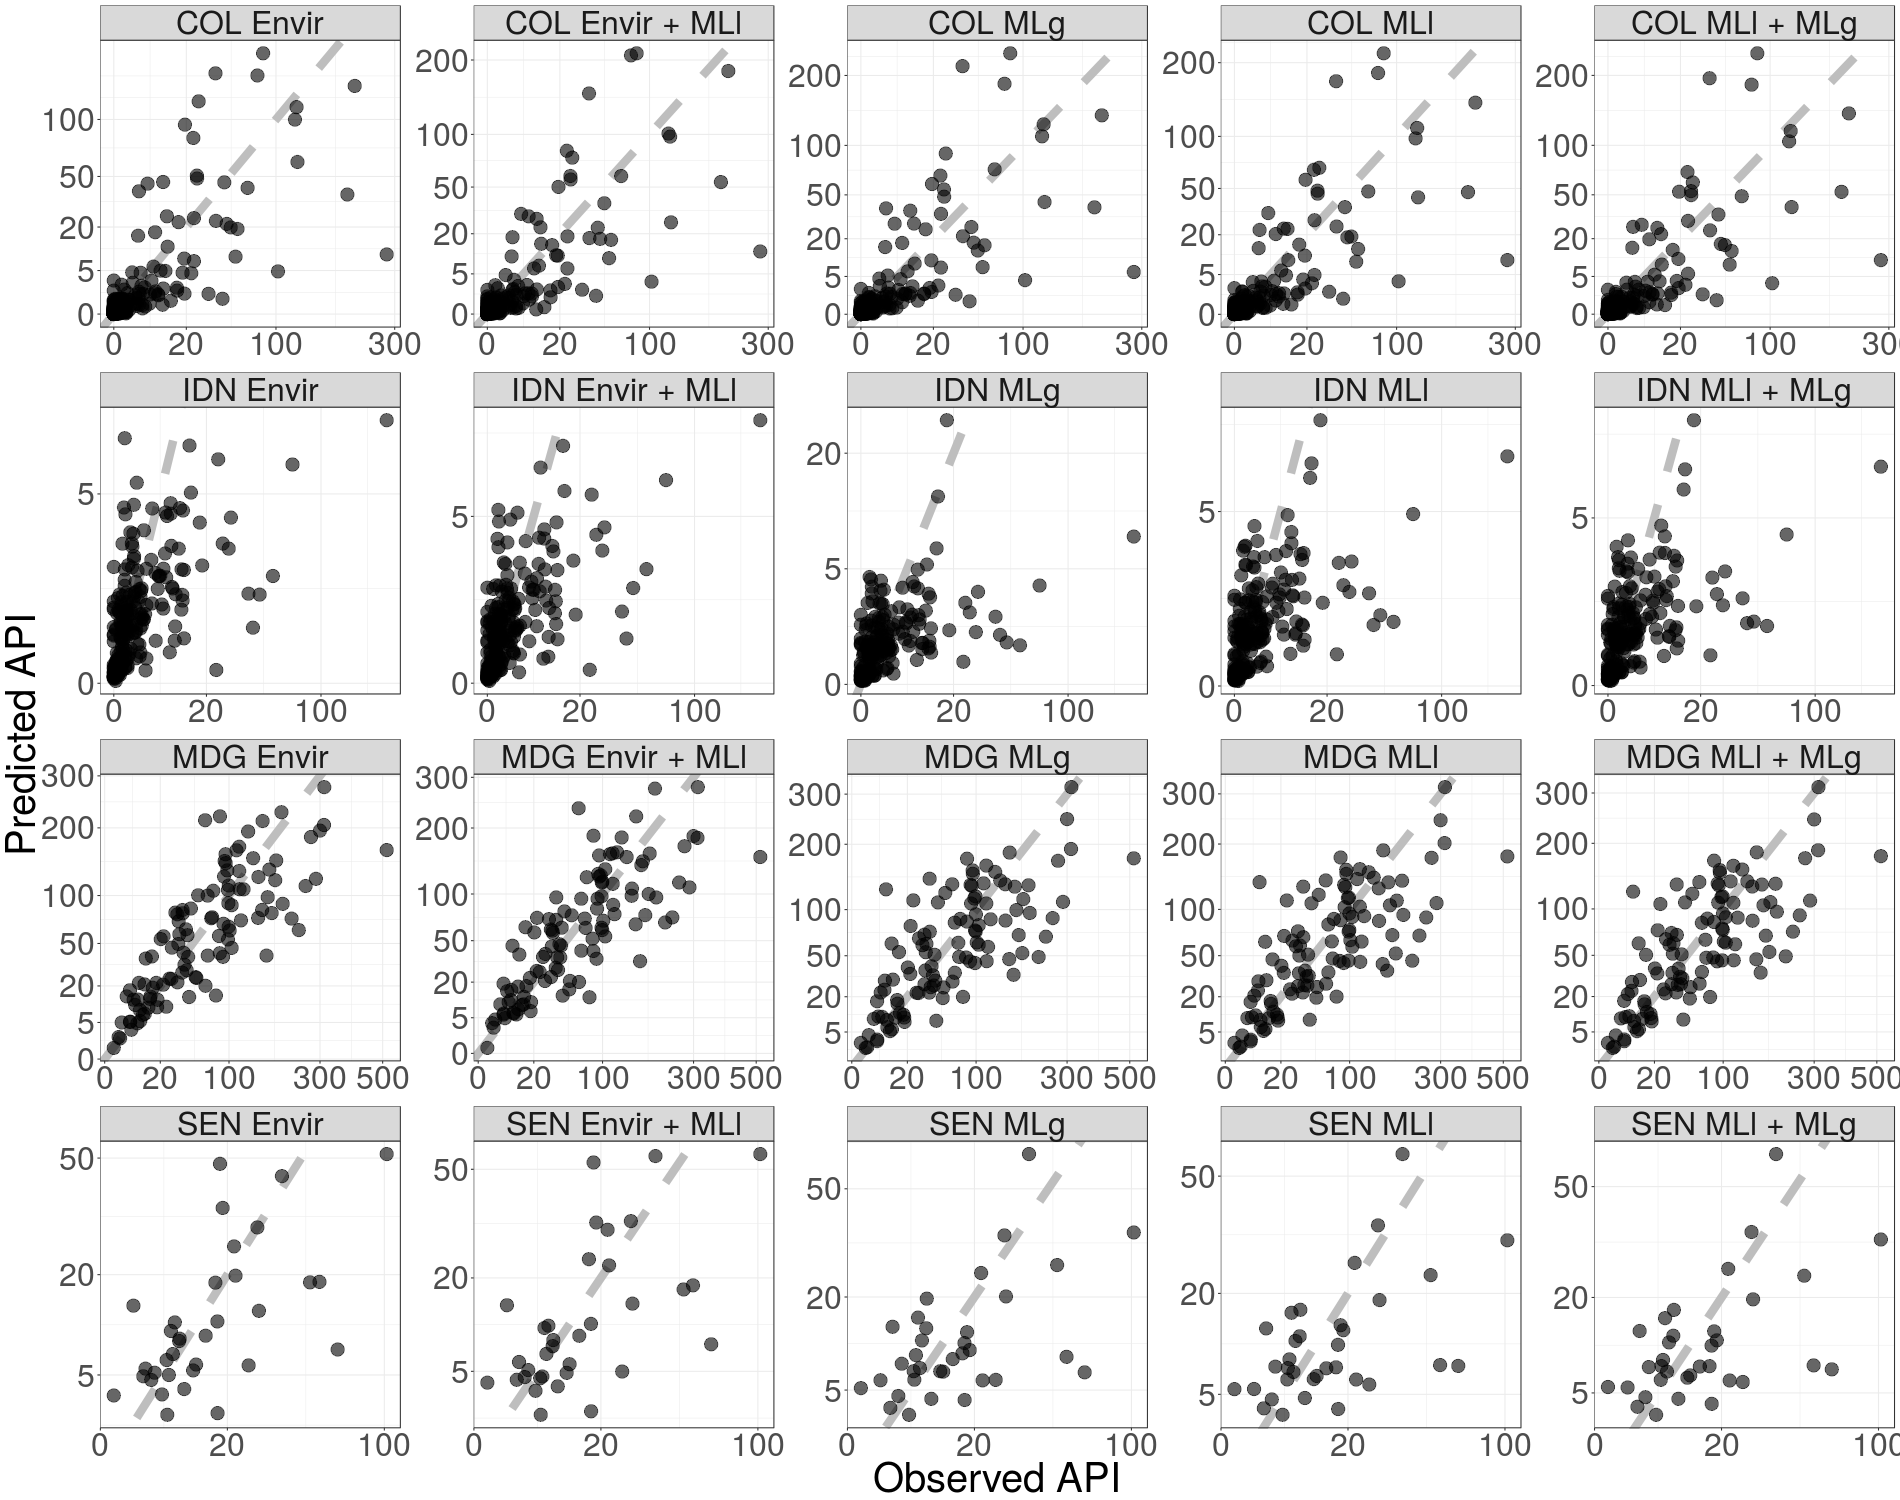
\includegraphics[width=\textwidth]{figs/cv1_scatter.png}
\caption{
  Observed data against predictions for cross-validation hold-out samples on a square root transformed scale.
}
\label{f:scatter1}
\end{figure}


\begin{figure}
  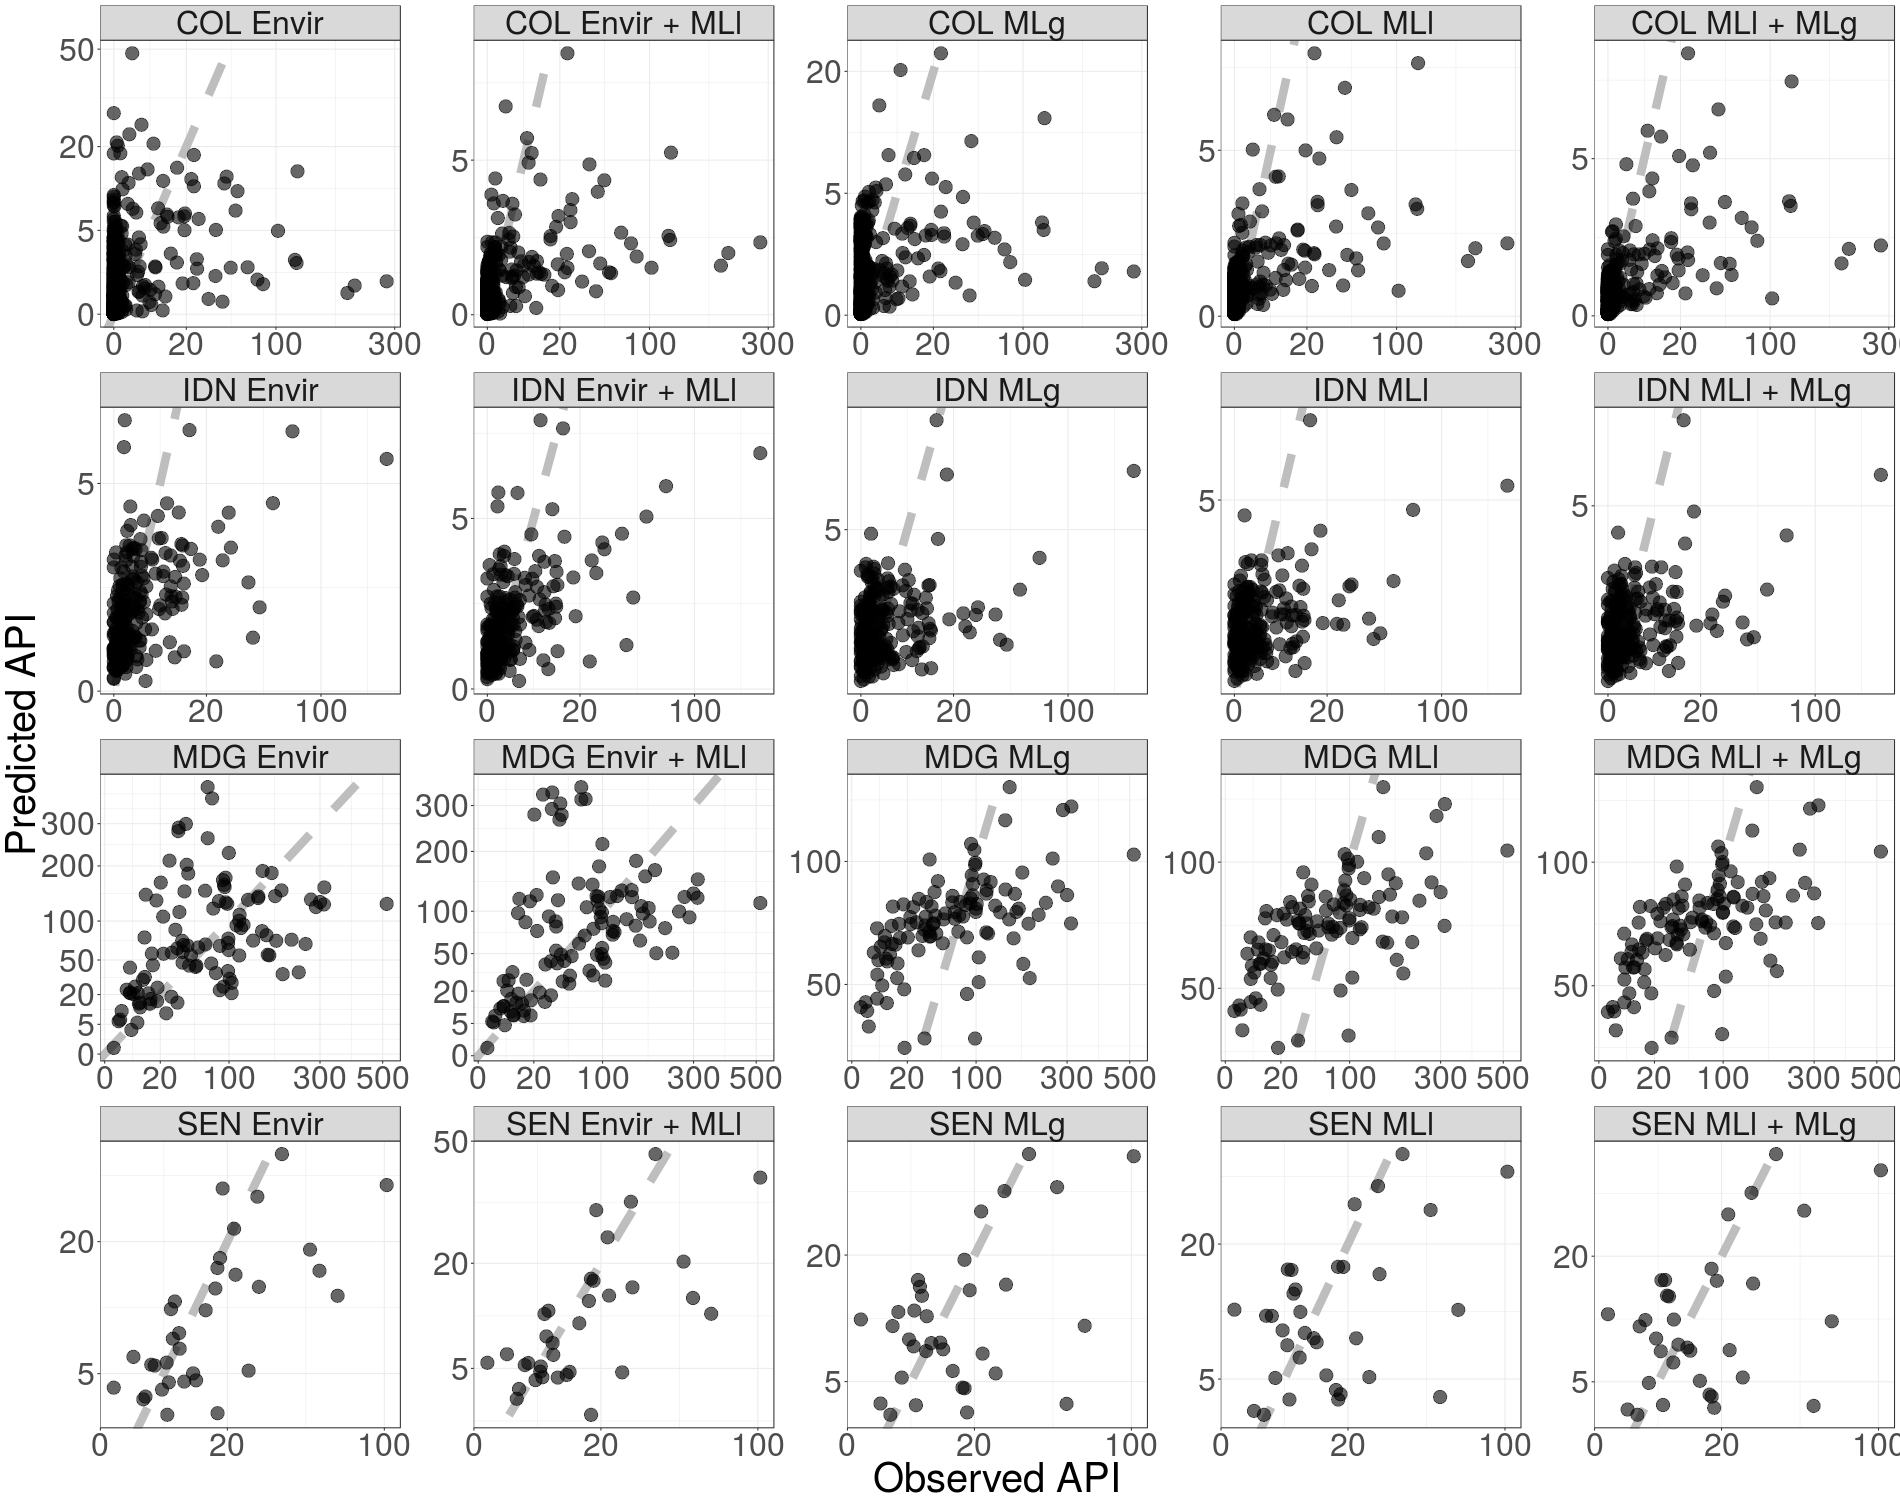
\includegraphics[width=\textwidth]{figs/cv2_scatter.png}
\caption{
  Observed data against predictions for cross-validation hold-out samples on a square root transformed scale.
}
\label{f:scatter2}
\end{figure}



\begin{figure}
\centering
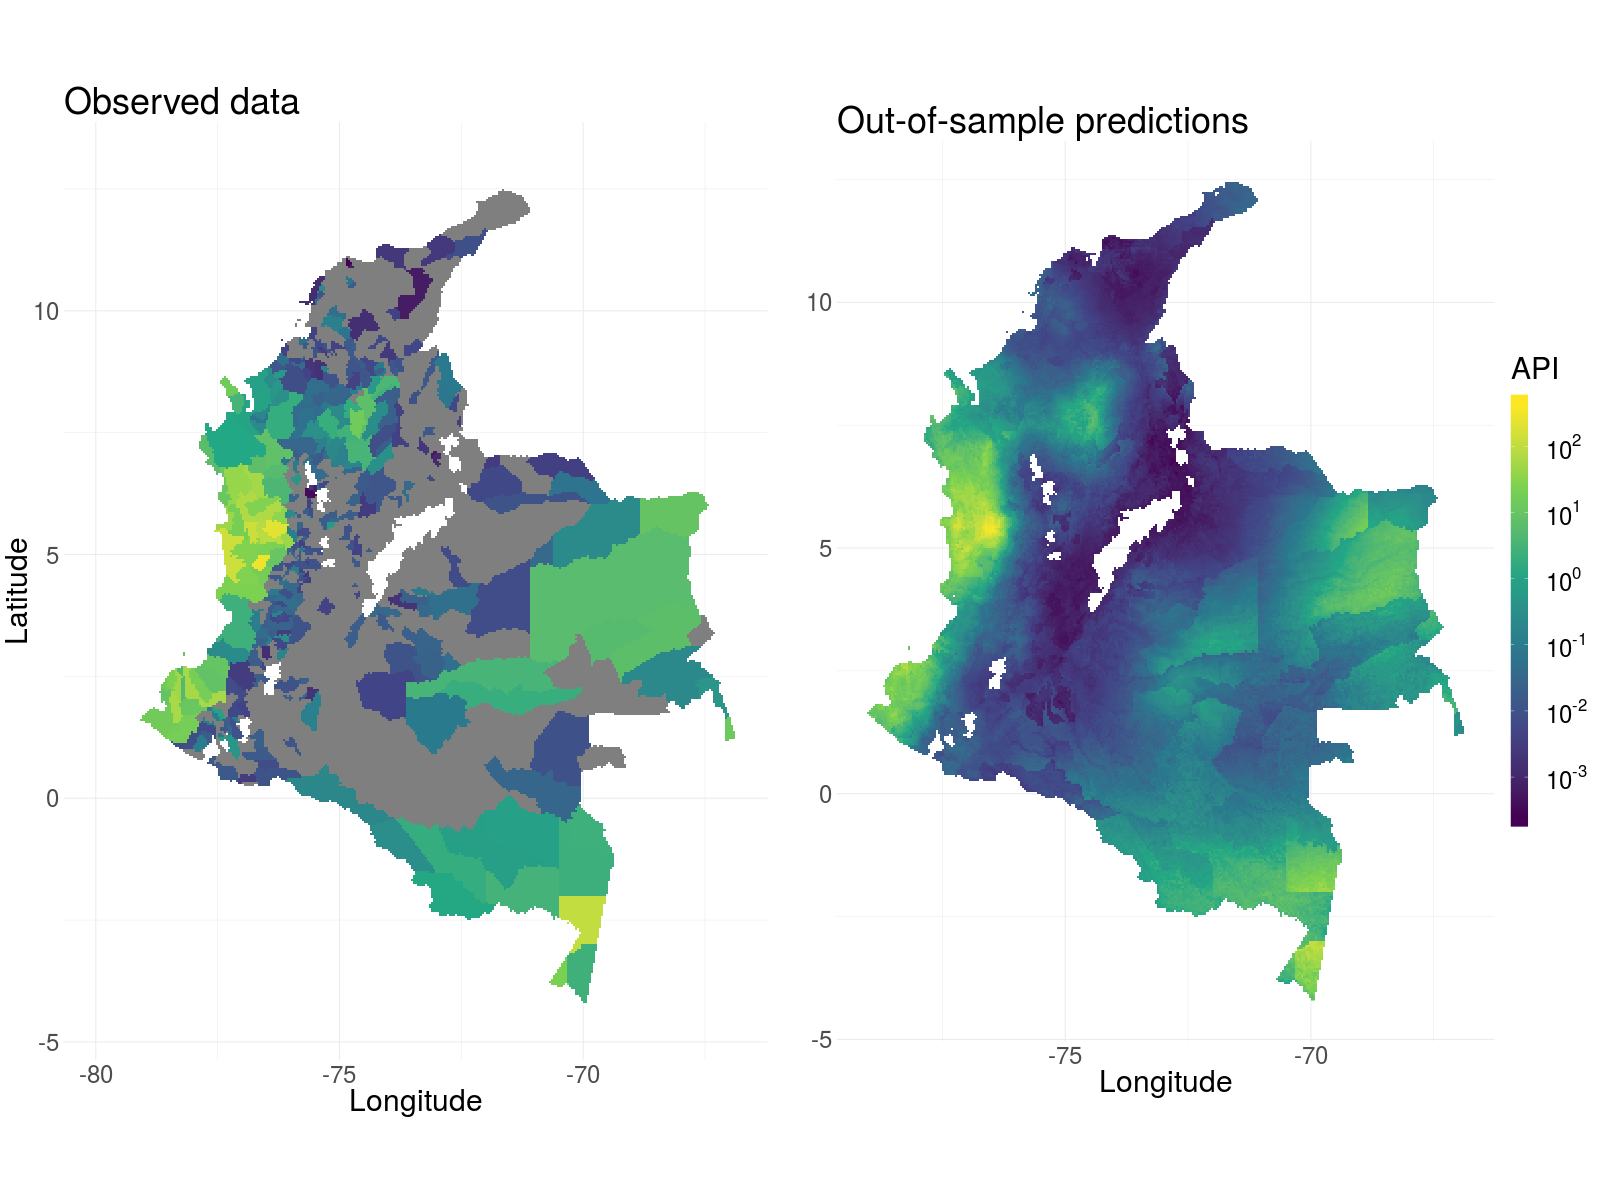
\includegraphics[trim={0 30mm 0 40mm}, width = 0.8\textwidth]{figs/col_obs_pred_map_ml.png} %\caption{Indonesia spatial crossvalidation} 
\caption{
  Left: Observed data for Colombia (grey for zero incidence). Right: Out-of-sample predictions for the random cross-validation, machine learning only model. For each cross-validation fold, predictions are made for the held out data which are then combined to make a single surface.
}
\label{f:map}
\end{figure}



\begin{table}
\caption{Machine learning model results and fitted parameters (i.e.\thinspace model weights) of the machine learning predictions only models (local only and global only). }
\centering
\small
\begin{tabular}{ll|rr|rr}
     Country          & Model &      RMSE\textsubscript{l} & $\beta_l$ & RMSE\textsubscript{g} & $\beta_g$ \\ \hline
Madagascar & RF & \textbf{0.100} & 0.538 &  \textbf{0.169} & \textbf{0.529}\\
Madagascar & GBM & 0.105 & \textbf{0.570} & 0.178& 0.432 \\
Madagascar & enet & 0.116 & 0.301 &0.233 & 0.262 \\
Madagascar & nnet & 0.113 & 0.033 &0.220 & 0.364 \\
Madagascar & ppr & 0.109 & 0.469 & 0.205 &  0.403\vspace{0.3cm}\\ 
Colombia & RF & \textbf{0.068} & 0.505 &  \textbf{0.169} & \textbf{0.522}\\
Colombia & GBM & 0.073 & \textbf{0.879} & 0.178& -0.231  \\
Colombia & enet & 0.070 & 0.079 &0.233 & 0.080 \\
Colombia & nnet & 0.070 & -0.008 &0.220 & 0.144 \\
Colombia & ppr & 0.070 & 0.530 & 0.205 &  0.468\vspace{0.3cm}\\
Senegal & RF & \textbf{0.092} & \textbf{0.339} & \textbf{0.169} & \textbf{0.425} \\
Senegal & GBM & 0.099 & 0.261& 0.178& 0.408 \\
Senegal & enet& 0.103 & 0.344  &0.233 & 0.205 \\
Senegal & nnet & 0.099 & 0.254 &0.220 & 0.190 \\
Senegal & ppr & 0.098 & 0.268& 0.205 &  0.126\vspace{0.3cm}\\
Indonesia & RF& \textbf{0.081} & 0.447 & \textbf{0.169} & 0.178\\
Indonesia & GBM & 0.085 & 0.357 & 0.178& 0.289 \\
Indonesia & enet & 0.091 & 0.303 &0.233 & \textbf{0.526} \\
Indonesia & nnet & 0.089 & \textbf{0.506} &0.220 & 0.316 \\
Indonesia & ppr & 0.089 & 0.364 & 0.205 &  0.089\vspace{0.3cm}\\

\end{tabular}
\label{t:mlresults}
\end{table}




\begin{table}[h!]
\caption{Covarage of 80\% credible intervals. Values outside 0.7--0.9 are shown in bold.}
\centering
\begin{tabular}{llrrrrr}
Country &  CV & Enviro & ML\textsubscript{l} &  Enviro + ML\textsubscript{l} & ML\textsubscript{g} & ML\textsubscript{l} + ML\textsubscript{g} \\
\hline 
 Colombia & Random & \textbf{0.28} & \textbf{0.28} & \textbf{0.29} & \textbf{0.29} & \textbf{0.29} \\
 Madagascar &  Random & 0.80 & 0.77& 0.75& 0.77& 0.76 \\
 Senegal & Random &0.79 & 0.79& 0.79& 0.79& 0.82 \\
 Indonesia & Random &0.80 & 0.81& 0.78& 0.79& 0.77  \\
 Colombia &  Spatial & \textbf{0.31} & \textbf{0.34}  & \textbf{0.32} & \textbf{0.34} & \textbf{0.34}  \\
 Madagascar & Spatial & \textbf{0.65} & 0.74& 0.70& 0.75 & 0.76   \\
 Senegal & Spatial & 0.85 & \textbf{0.91}& 0.85& \textbf{0.94} & 0.85  \\
  Indonesia & Spatial & 0.80 & 0.78& 0.78& 0.76& 0.75  \\
\end{tabular}
\label{t:results2}
\end{table}






\begin{table}
\caption{Fitted regression parameters of the environmental and machine learning covariates for thee models: just environmental variables, just local machine learning models and the combination of the two.}
\centering
\tiny
\begin{tabular}{ll|rrr}
Country    & Variable &  $\beta_{enviro}$   & $\beta_l$ & $\beta_{enviro+l}$\\ \hline
Madagascar & LST mean & 0.17 &  &  -0.01\\
Madagascar & EVI & 0.32 &  & -0.04 \\
Madagascar & TSI & 0.42 &  &0.06  \\
Madagascar & access & 0.34 &  &0.00  \\
Madagascar & Elev & -0.14 &  & 0.00\\ 
Madagascar & LST sd & -0.78 &  &-0.04  \\
Madagascar & VIIRS & -0.1 &  &-0.52  \\
Madagascar & TCW & -0.22 &  & -0.06\\ 
Madagascar & RF &  & 0.29 &  0.01\\
Madagascar & GBM &  & 0.52 & 0.25 \\
Madagascar & enet &  & 0.31 &0.09  \\
Madagascar & nnet &  & 0.43 &0.14  \\
Madagascar & ppr &  & 0.49 & 0.22\vspace{0.2cm}\\ 
Colombia & LST mean &-0.12  &  & -0.22\\
Colombia & EVI &  -0.08&  & 0.17\\
Colombia & TSI &  0.54&  & -0.06\\
Colombia & access &  0.35&  &0.00 \\
Colombia & Elev &  0.47&  & 0.00\\
Colombia & LST sd & -0.11 &  & -0.10\\
Colombia & VIIRS & 0.24 &  & 0.01\\
Colombia & TCW &  0.21&  & 0.00\\
Colombia & RF &  & 0.36 & -0.18\\
Colombia & GBM &  & 0.54 & 0.26\\
Colombia & enet &  & 0.32 & -0.34\\
Colombia & nnet &  &0.33  & -0.09\\
Colombia & ppr &  & 0.54 & 0.01\vspace{0.2cm}\\
Senegal & LST mean &-0.04  &  &-0.02\\
Senegal & EVI &  0.33&  & 0.30\\
Senegal & TSI &  -0.58&  &  -0.59\\
Senegal & access & -0.03 &  &  -0.05\\
Senegal & Elev &  0.42&  &0.37\\ 
Senegal & LST sd &  0.21&  & 0.10 \\
Senegal & VIIRS &  0.13&  &  0.13\\
Senegal & TCW & 0.08 &  &-0.01\\ 
Senegal & RF &  & 0.34 &  0.20\\
Senegal & GBM &  &  0.28& 0.05\\
Senegal & enet &  &  0.27&  -0.05\\
Senegal & nnet &  & 0.29 &-0.09 \\
Senegal & ppr &  &  0.35& 0.25\vspace{0.2cm}\\
Indonesia & LST mean & -0.32 &  &-0.34\\
Indonesia & EVI &  0.49&  & 0.36\\
Indonesia & TSI &  0.58&  &0.52\\
Indonesia & access &0.33 &  & 0.06 \\
Indonesia & Elev& -0.06&  &-0.13\\ 
Indonesia & LST sd & -0.23 &  & -0.33\\
Indonesia & VIIRS &  -0.12&  & 0.03\\
Indonesia & TCW& 0.12 &  &0.10\\ 
Indonesia & RF &  & 0.32 & 0.06\\
Indonesia & GBM &  &  0.38&0.03\\
Indonesia & enet &  &  0.49&  0.56\\
Indonesia & nnet &  &  0.36&  0.18\\
Indonesia & ppr &  &  0.45& 0.32\\



\end{tabular}
\label{t:mlresults}
\end{table}



\section{Discussion}

\section{Conclusions}

Overall, our experiments suggest that using predictions from machine learning models trained on prevalence points provides more accurate predictions than using environmental covariates when fitting disaggregation models of malaria incidence.
This increased performance comes despite the data being on different scales, the data being measurements of different aspects of malaria transmission and despite the imperfect model we have used to translate between the two scales.
However, the reduced model accuracy in the spatial cross-validation schemes, relative to the random cross-validation scheme, highlights that better spatial coverage of data would improve predictions more than the improved model we have suggested.

Due to the low power of typical aggregated incidence datasets, previous analyses using disaggregation regression used a small number of covariates \citep{sturrock2014fine}.
However, as models such as Random Forest and elastic net can robustly handle high dimensional data, future work could include many more covariates, potentially increasing predictive performance.

% this method is an improvement
% still reliant on spatial field

% allows broad suite of covariates

% sum to one stacking
% global ml models, local experts

While the approach presented here is related to stacking, it differs in that we have not constrained the regression parameters to be positive nor included a sum-to-one constraint i.e.\thinspace the result is not simply a weighted average of the level zero model predictions.
We did not include these constraints because the base models and the meta model are trained on response data on different scales.
However, future work could examine whether using a positive constraint on the regression parameters improves performance.

Another area of potential improvement is varying the data used to train the base level learners.
Here we only used data from the region of interest.
However, the global dataset is much larger than these subsets.
Training some base level models on local data and some on the global dataset and then combining predictions from all these models has potential to further improve model performance.

\section*{Acknowledgments}
The authors acknowledge the National Malaria Control Programme of Madagascar for sharing their routine case data for this analysis.

\bibliography{Malaria} 
\bibliographystyle{apalike}





\end{document}









